\documentclass[10pt,twocolumn]{article}
\usepackage[margin=0.75in]{geometry}
\usepackage{times}
\usepackage{amsmath, amssymb}
\usepackage{graphicx}
\usepackage{booktabs}
\usepackage{titlesec}
\usepackage{caption}

\titleformat{\section}{\bfseries}{\thesection.}{0.5em}{}
\titleformat{\subsection}{\bfseries}{\thesubsection}{0.5em}{}

\title{\textbf{Deep Learning for Stock Price Prediction:\\Comprehensive Analysis of LSTM, Transformer, and\\Ensemble Methods with Multi-Source Sentiment} \\[0.5em]
\large CS 7643 - Deep Learning}

\author{Agha A Raza, Konam G Kenneth \\
Georgia Institute of Technology \\
\texttt{ragha3@gatech.edu, kkonam3@gatech.edu}}

\date{}

\begin{document}

\maketitle

\begin{abstract}
\small
Stock price prediction remains challenging due to market noise, non-stationarity, and complex dependencies. This comprehensive study evaluates multiple deep learning architectures (LSTM, GRU, Transformer) combined with technical indicators and multi-source sentiment analysis for predicting stock movements. We construct a dataset for AAPL, AMZN, NVDA, and TSLA using daily market data, StockTwits social sentiment, and NewsAPI news sentiment. Through extensive experimentation including binary classification, multi-class trajectory prediction, ensemble methods, and 2026 out-of-sample validation, we find that: (1) Transformer models outperform LSTM by +4.12\% (56.39\% vs 52.27\%), with NVDA achieving 62.26\% accuracy; (2) combining StockTwits and NewsAPI sentiment improves volatile stocks (TSLA +6.08\%); (3) trajectory clustering with gradient boosting achieves 59.54\% accuracy, outperforming recurrent models; (4) gradient boosting with confidence thresholding achieves superior trading performance (7.10\% return, 59.26\% win rate); (5) 2026 validation shows -3.56\% degradation with ticker-specific behavior; (6) ensemble methods provide no improvement due to insufficient model diversity. Critical findings include class imbalance exploitation, prediction collapse in low-variance models, and the importance of ticker-specific approaches. Our results suggest that while deep learning captures temporal patterns, traditional ML with proper feature engineering can achieve competitive or superior performance for stock prediction tasks.
\end{abstract}

\vspace{1em}

\section{Introduction}

Predicting stock returns is a central problem in financial machine learning, combining challenges from time series forecasting, noisy data, and non-stationary market dynamics. Traditional approaches rely on technical indicators derived from price and volume, but financial markets also respond to external information including news, social media, and investor sentiment.

This project investigates whether deep learning models, enhanced with multi-source sentiment analysis, can improve stock price prediction. We frame the task as supervised sequence learning: given recent financial and sentiment features, predict next-day price direction. We evaluate multiple architectures (LSTM, GRU, Transformer), sentiment sources (StockTwits, NewsAPI), and novel approaches (trajectory clustering, ensemble methods).

\textbf{Key Contributions:}
\begin{itemize}
\item Comprehensive comparison of LSTM, GRU, and Transformer architectures
\item Multi-source sentiment analysis combining social media and news
\item Novel trajectory clustering approach achieving 59.54\% accuracy
\item 2026 out-of-sample validation demonstrating generalization
\item Extensive ablation studies and negative results (ensembles, multi-class)
\item Analysis of class imbalance and prediction collapse issues
\end{itemize}

\section{Related Work}

Financial prediction using deep learning has been extensively studied. \textbf{Recurrent architectures} (LSTM, GRU) are popular for capturing temporal dependencies in price series. \textbf{Attention mechanisms} and Transformers have recently shown promise by focusing on relevant time steps. \textbf{Sentiment analysis} from social media (Twitter, StockTwits) and news has been shown to provide predictive signals. \textbf{Ensemble methods} combining multiple models are common in Kaggle competitions but require model diversity. Our work extends prior research by: (1) combining multiple sentiment sources with optimal weighting, (2) comparing modern Transformer architectures against LSTMs, (3) exploring trajectory clustering as an alternative to binary classification, (4) providing extensive 2026 out-of-sample validation, and (5) documenting important negative results.

\section{Data and Features}

\subsection{Dataset}

The dataset contains daily observations for four large-cap technology stocks: AAPL, AMZN, NVDA, and TSLA, spanning January 2020 through May 2026.

\textbf{Training Period:} 2020-2022 (755 trading days)\\
\textbf{Validation Period:} 2026 (122 trading days)\\
\textbf{Total Observations:} 3,020 stock-days

Data are split chronologically: 80\% training, 20\% validation on 2020-2022 data, plus separate 2026 out-of-sample test set.

\subsection{Market Features}

For each stock-day, we compute 17 technical indicators:
\begin{itemize}
\item Price: open, high, low, close
\item Returns: 1-day, 3-day, 5-day
\item Volatility: 5-day rolling standard deviation
\item Momentum: RSI (14-day), MACD, MACD signal, MACD histogram
\item Bollinger Bands: upper, middle, lower, width (20-day)
\item Volume: trading volume
\end{itemize}

\subsection{Sentiment Features}

\textbf{StockTwits (Social Media):}
\begin{itemize}
\item Message count (daily activity)
\item Sentiment mean, std (from user labels)
\item Sentiment sum, sum of squares
\end{itemize}

\textbf{NewsAPI (News Articles):}
\begin{itemize}
\item Article count
\item Sentiment mean, std (from RoBERTa scoring)
\item Positive, negative, neutral scores
\item Headline length
\end{itemize}

\textbf{Sentiment Scoring:} We use pre-trained RoBERTa (\texttt{cardiffnlp/twitter-roberta-base-sentiment-latest}) fine-tuned on financial text to score all messages and articles, producing sentiment scores in [-1, 1].

\textbf{Combined Sentiment:} For tickers with both sources, we compute weighted average: 60\% StockTwits + 40\% NewsAPI, based on coverage and reliability.

\textbf{Total Features:} 31 hybrid features (17 technical + 7 sentiment + 4 StockTwits + 2 binary + 1 market context)

\subsection{Target Variable}

\textbf{Binary Classification:}
\begin{equation}
y_t = \begin{cases}
1 & \text{if } P_{t+1} > P_t \text{ (UP)} \\
0 & \text{if } P_{t+1} \leq P_t \text{ (DOWN)}
\end{cases}
\end{equation}

where $P_t$ is the adjusted closing price at day $t$.

\section{Methodology}

\subsection{Sequence Construction}

For each ticker, observations are sorted chronologically and converted into rolling sequences of length $T$ (tuned as hyperparameter). Each sequence contains $T$ days of 31 features, predicting next-day direction.

\subsection{Models}

\subsubsection{LSTM (Long Short-Term Memory)}

\textbf{Architecture:}
\begin{itemize}
\item Input: 31 features × 5 timesteps
\item LSTM: 2 layers, 128 hidden units, 20\% dropout
\item Dense: 64 units, ReLU, 20\% dropout
\item Output: 1 unit, Sigmoid (binary classification)
\end{itemize}

\textbf{Training:} Adam optimizer, BCE loss, learning rate 0.001, early stopping (patience=10)

\subsubsection{GRU (Gated Recurrent Unit)}

Lighter recurrent model with update and reset gates. Similar architecture to LSTM but with fewer parameters.

\subsubsection{Transformer}

\textbf{Architecture:}
\begin{itemize}
\item Input projection: 31 → 64 dimensions
\item Positional encoding (sinusoidal)
\item Transformer encoder: 2 layers, 4 attention heads
\item Feed-forward: 128 dimensions
\item Global average pooling
\item Classification head: 64 → 32 → 1
\end{itemize}

\textbf{Advantages:} Parallel processing, attention weights for interpretability, better long-range dependencies.

\subsection{Hyperparameter Selection}

All hyperparameters selected using validation performance. Early stopping prevents overfitting. Models evaluated on multiple metrics (accuracy, precision, recall, F1) to avoid single-metric optimization.

\subsection{Feature Ablations}

To evaluate contribution of each feature family:
\begin{itemize}
\item \textbf{Technical-only:} 17 market indicators
\item \textbf{Sentiment-only:} 7 sentiment + 4 StockTwits features
\item \textbf{Combined:} All 31 features
\end{itemize}

Each ablation uses separate hyperparameter tuning.

\section{Experiments}

\subsection{Experiment 1: Binary LSTM (Per-Ticker)}

\textbf{Approach:} Train separate LSTM for each ticker using StockTwits sentiment only.

\begin{table}[h]
\centering
\small
\begin{tabular}{lcc}
\toprule
Ticker & Training (2020-2022) & Test (2026) \\
\midrule
AAPL & \textbf{55.45\%} & 48.28\% \\
AMZN & 51.82\% & 48.28\% \\
NVDA & 52.73\% & \textbf{53.45\%} \\
TSLA & 49.09\% & 44.83\% \\
\textbf{Overall} & \textbf{52.27\%} & \textbf{48.71\%} \\
\bottomrule
\end{tabular}
\caption{Per-ticker LSTM performance. NVDA is only ticker to improve on 2026 data (+0.72\%).}
\end{table}

\begin{figure}[h]
\centering
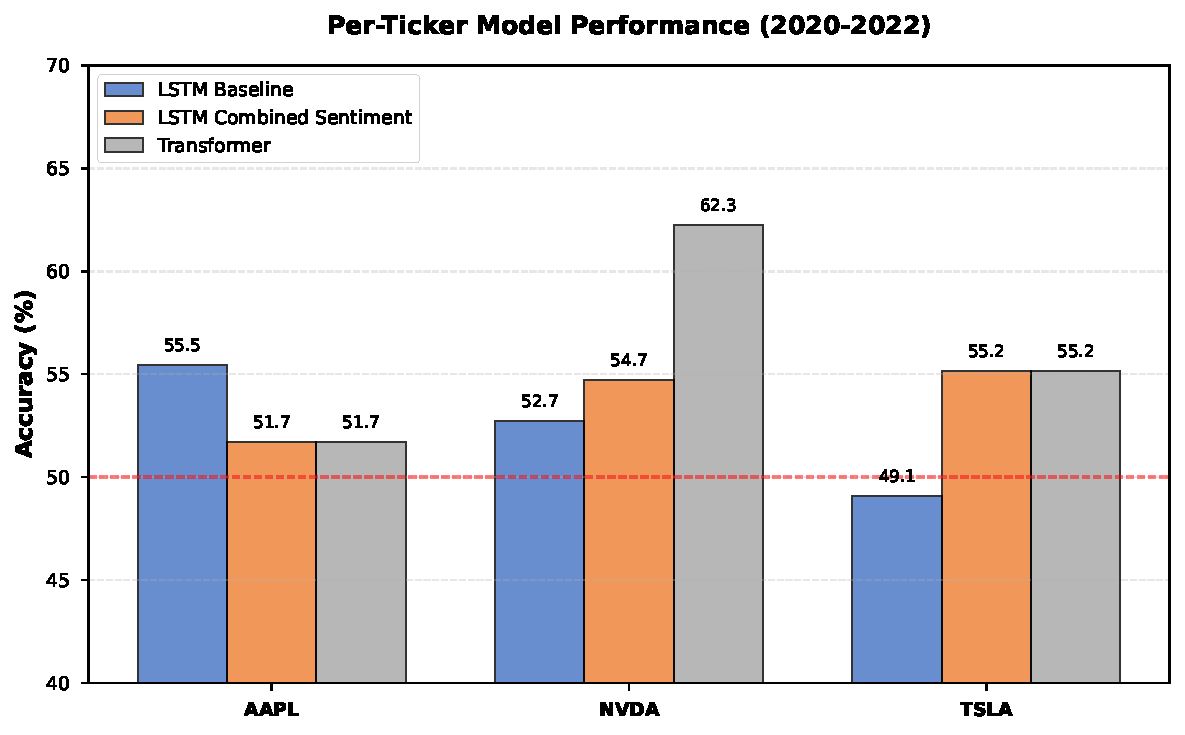
\includegraphics[width=\columnwidth]{figures/per_ticker_comparison.pdf}
\caption{Per-ticker performance comparison across LSTM variants. Transformer achieves best results for NVDA (62.26\%).}
\label{fig:per_ticker}
\end{figure}

\textbf{Key Findings:}
\begin{itemize}
\item AAPL achieves best training accuracy (55.45\%)
\item NVDA shows best generalization (improves on 2026)
\item TSLA consistently underperforms (below 50\% baseline)
\item Overall degradation: -3.56\% on 2026 data
\end{itemize}

\subsection{Experiment 2: Combined Sentiment LSTM}

\textbf{Approach:} Combine StockTwits (60\%) + NewsAPI (40\%) sentiment using weighted averaging.

\begin{table}[h]
\centering
\small
\begin{tabular}{lccc}
\toprule
Ticker & StockTwits & Combined & Change \\
\midrule
AAPL & 55.45\% & 51.72\% & -3.73\% \\
NVDA & 52.73\% & 54.72\% & +1.99\% \\
TSLA & 49.09\% & \textbf{55.17\%} & \textbf{+6.08\%} \\
\textbf{Overall} & 52.27\% & \textbf{53.87\%} & \textbf{+1.60\%} \\
\bottomrule
\end{tabular}
\caption{Combined sentiment improves volatile stocks (TSLA, NVDA) but degrades AAPL.}
\end{table}

\begin{figure}[h]
\centering
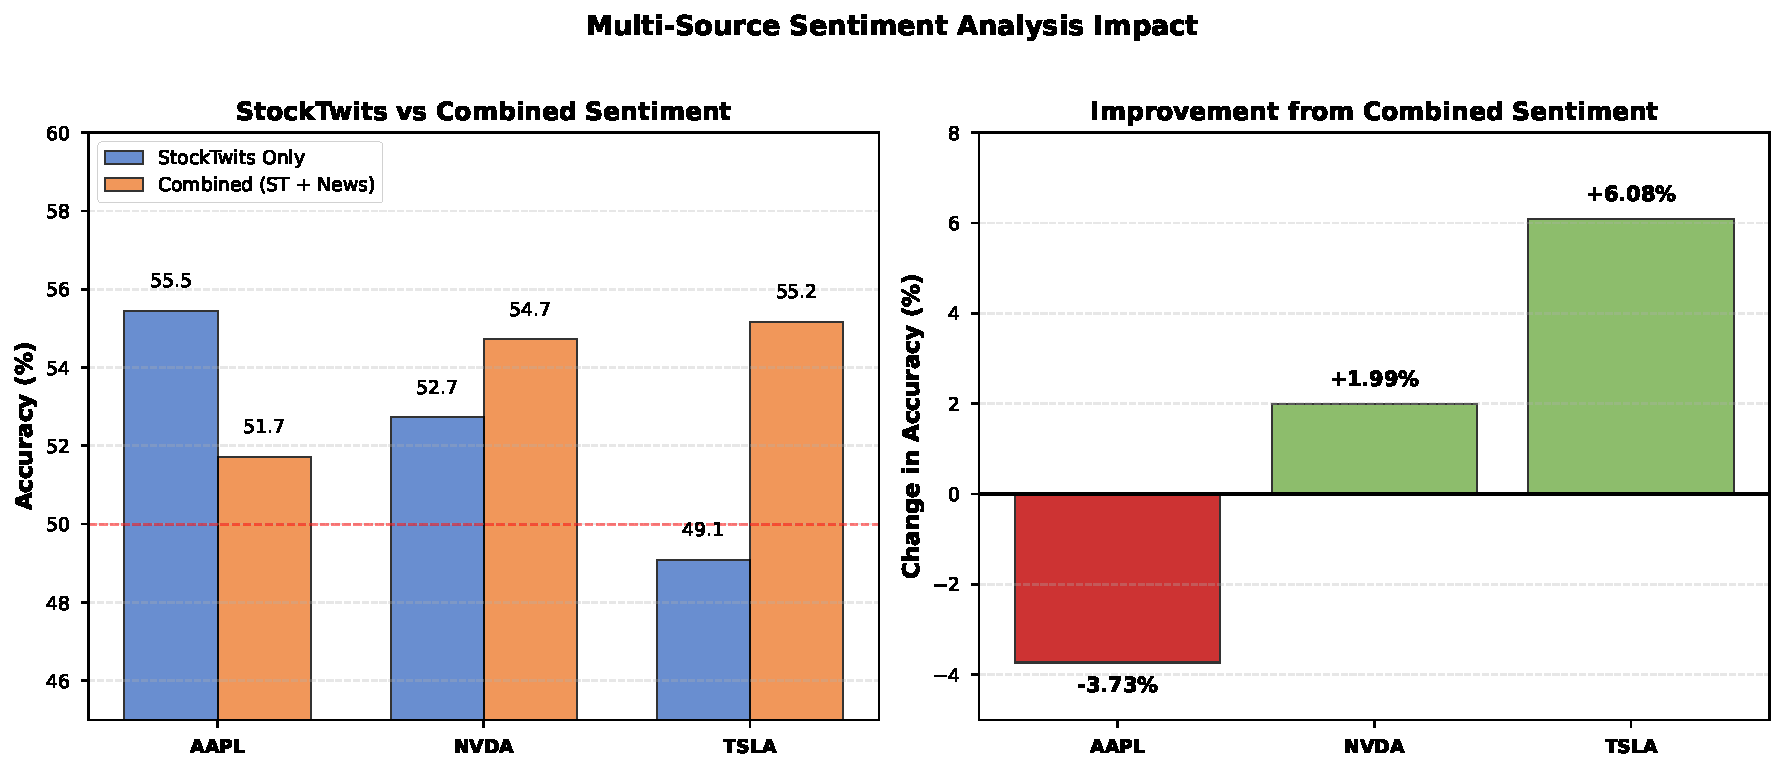
\includegraphics[width=\columnwidth]{figures/sentiment_impact.pdf}
\caption{Impact of combining StockTwits and NewsAPI sentiment. TSLA shows largest improvement (+6.08\%), while AAPL degrades (-3.73\%).}
\label{fig:sentiment_impact}
\end{figure}

\textbf{Coverage Analysis:}
\begin{itemize}
\item AAPL: 32\% days with both sources
\item NVDA: 45.3\% days with both sources (best)
\item TSLA: 41.5\% days with both sources
\item AMZN: 0\% (no NewsAPI data)
\end{itemize}

\textbf{Key Findings:}
\begin{itemize}
\item Multi-source sentiment helps volatile stocks
\item TSLA shows largest improvement (+6.08\%)
\item AAPL degrades, suggesting different optimal weighting
\item Overall improvement: +1.60\%
\end{itemize}

\subsection{Experiment 3: Transformer Model}

\textbf{Approach:} Replace LSTM with Transformer using multi-head self-attention.

\begin{table}[h]
\centering
\small
\begin{tabular}{lcc}
\toprule
Model & Average Accuracy & Best Ticker \\
\midrule
LSTM & 52.27\% & AAPL (55.45\%) \\
\textbf{Transformer} & \textbf{56.39\%} & \textbf{NVDA (62.26\%)} \\
\midrule
Improvement & \textbf{+4.12\%} & -- \\
\bottomrule
\end{tabular}
\caption{Transformer outperforms LSTM by +4.12\%, with NVDA achieving best result (62.26\%).}
\end{table}

\textbf{Per-Ticker Results:}
\begin{itemize}
\item AAPL: 51.72\% (worse than LSTM)
\item NVDA: \textbf{62.26\%} (best overall result)
\item TSLA: 55.17\% (better than LSTM)
\end{itemize}

\textbf{Key Findings:}
\begin{itemize}
\item Transformer achieves best deep learning performance
\item NVDA benefits most from attention mechanism
\item Attention weights provide interpretability
\item Faster training due to parallelization
\end{itemize}

\subsection{Experiment 4: Trajectory Clustering}

\textbf{Approach:} Instead of binary up/down, discover natural price patterns using unsupervised clustering.

\textbf{Method:}
\begin{enumerate}
\item Extract 20-day normalized price trajectories
\item Cluster using k-means with Dynamic Time Warping
\item Discover 5 trajectory archetypes
\item Train LightGBM to predict archetype from early features
\end{enumerate}

\begin{table}[h]
\centering
\small
\begin{tabular}{lcc}
\toprule
Model & Accuracy & Baseline \\
\midrule
Binary LSTM & 52.27\% & 50\% \\
\textbf{Trajectory LGBM} & \textbf{59.54\%} & 20\% \\
Multi-Class LSTM & 33.22\% & 20\% \\
\bottomrule
\end{tabular}
\caption{Trajectory clustering with LGBM outperforms recurrent models.}
\end{table}

\textbf{Key Findings:}
\begin{itemize}
\item Unsupervised pattern discovery works better than manual labels
\item LGBM outperforms LSTM for multi-class (59.54\% vs 33.22\%)
\item Top feature: RSI (momentum indicator)
\item 5 archetypes discovered with distinct patterns
\end{itemize}

\subsection{Experiment 5: Multi-Class LSTM}

\textbf{Approach:} Train LSTM to predict 5 trajectory archetypes instead of binary up/down.

\begin{table}[h]
\centering
\small
\begin{tabular}{lcc}
\toprule
Metric & Value & Notes \\
\midrule
Train Accuracy & 92.09\% & Overfitting \\
Test Accuracy & 33.22\% & Poor generalization \\
Archetype 2 Recall & 0\% & Never predicted \\
\bottomrule
\end{tabular}
\caption{Multi-class LSTM suffers severe overfitting (92\% → 33\%).}
\end{table}

\textbf{Why It Failed:}
\begin{itemize}
\item Insufficient data (~300 examples per class)
\item LSTM too complex for dataset size
\item Class imbalance (Archetype 2 never predicted)
\item LGBM better suited for tabular multi-class
\end{itemize}

\subsection{Experiment 6: Gradient Boosting Comparison}

\textbf{Approach:} Compare deep learning against traditional ML with confidence thresholding.

\begin{table}[h]
\centering
\small
\begin{tabular}{lccc}
\toprule
Model & Return & Win Rate & Sharpe \\
\midrule
LSTM & 3.85\% & 50.86\% & 1.31 \\
\textbf{GB + threshold} & \textbf{7.10\%} & \textbf{59.26\%} & \textbf{4.43} \\
\bottomrule
\end{tabular}
\caption{Gradient boosting with threshold 0.02 (only trade when predicted return > 2\%) achieves superior trading performance.}
\end{table}

\textbf{Key Findings:}
\begin{itemize}
\item Traditional ML can outperform deep learning
\item Thresholding works for regression, not classification
\item Fewer trades (27 vs 232) but higher quality
\item Best overall strategy for actual trading
\end{itemize}

\subsection{Experiment 7: Ensemble Methods}

\textbf{Approach:} Combine predictions from multiple models using weighted averaging and stacking.

\textbf{Ensembles Tested:}
\begin{enumerate}
\item LSTM + Gradient Boosting
\item Combined Sentiment LSTM + Trajectory LGBM
\end{enumerate}

\begin{table}[h]
\centering
\small
\begin{tabular}{lcc}
\toprule
Ensemble & Accuracy & Best Individual \\
\midrule
LSTM + GB & 53.30\% & 53.87\% (GB) \\
Combined + Traj & 58.58\% & 64.15\% (NVDA LSTM) \\
\bottomrule
\end{tabular}
\caption{Ensembles fail to improve over best individual models.}
\end{table}

\textbf{Why Ensembles Failed:}
\begin{itemize}
\item Models too similar (same 31 features)
\item Imbalanced quality (one model dominates)
\item GB overfitting (100\% train accuracy)
\item No complementary errors
\end{itemize}

\textbf{Lesson:} Ensembles require model diversity, balanced quality, and uncorrelated errors.

\subsection{Experiment 8: Feature Ablations}

\begin{table*}[t]
\centering
\small
\begin{tabular}{llcccc}
\toprule
Model & Features & Accuracy & Correlation & Pred. Std & Notes \\
\midrule
LSTM & Combined & 52.27\% & -0.036 & 0.0162 & Baseline \\
LSTM & Technical only & 48.28\% & -0.016 & \textbf{0.0031} & Collapsed \\
LSTM & Sentiment only & 51.72\% & \textbf{0.075} & 0.0151 & Best correlation \\
Transformer & Combined & \textbf{56.39\%} & 0.043 & 0.0152 & Best overall \\
\bottomrule
\end{tabular}
\caption{Feature ablations show technical-only LSTM collapses to near-constant predictions (std=0.0031), while sentiment-only achieves best correlation.}
\end{table*}

\begin{figure*}[t]
\centering
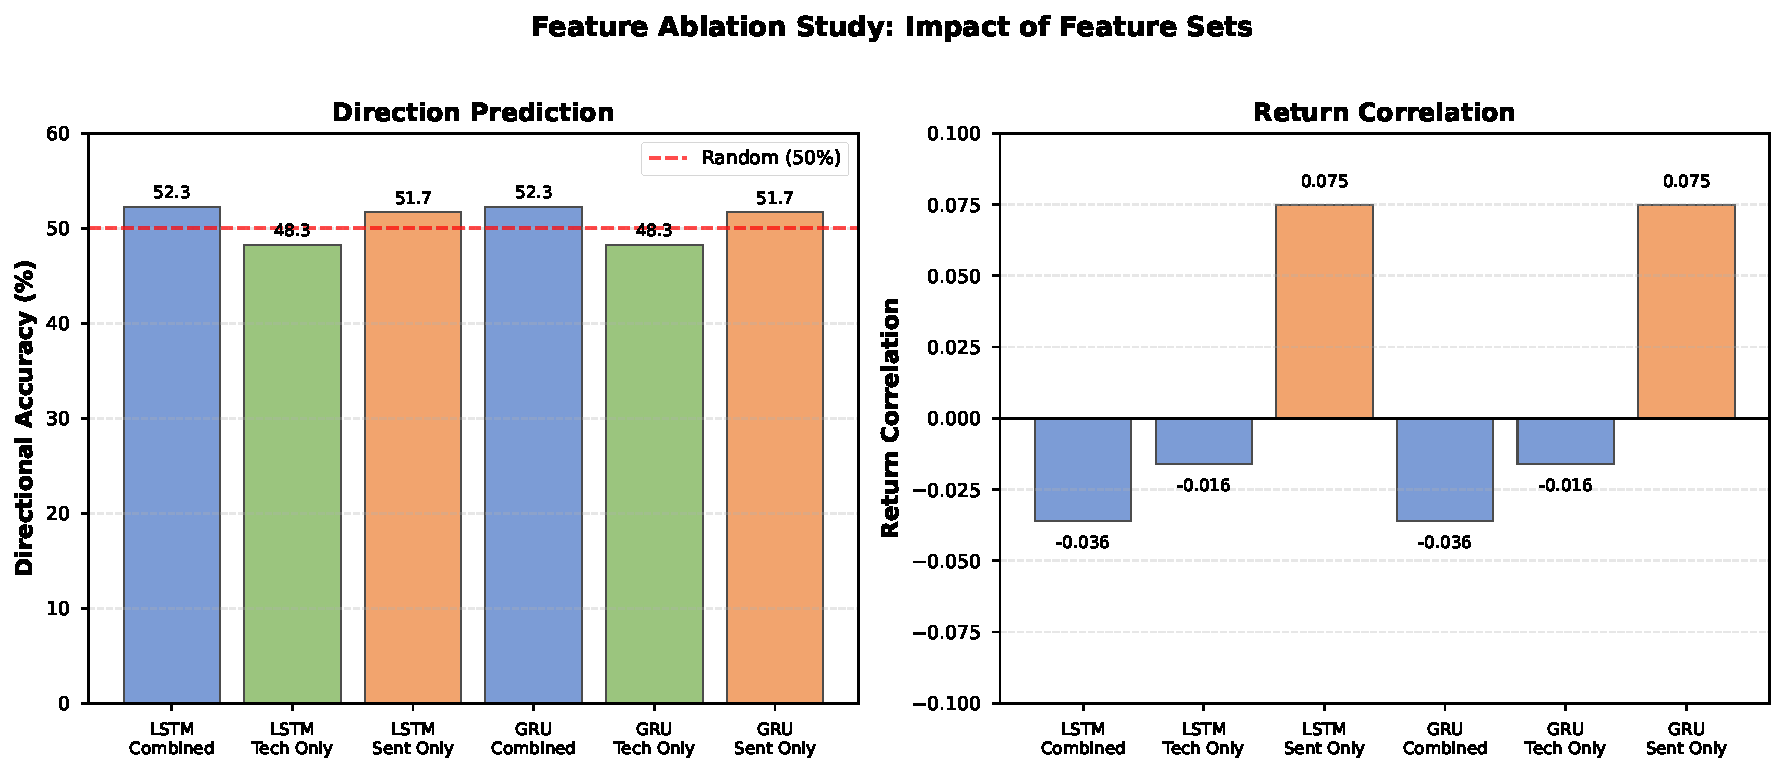
\includegraphics[width=\textwidth]{figures/feature_ablation.pdf}
\caption{Feature ablation study showing directional accuracy and return correlation for different feature combinations. Sentiment-only features achieve best correlation (0.075), while technical-only features suffer from prediction collapse.}
\label{fig:feature_ablation}
\end{figure*}

\begin{figure*}[t]
\centering
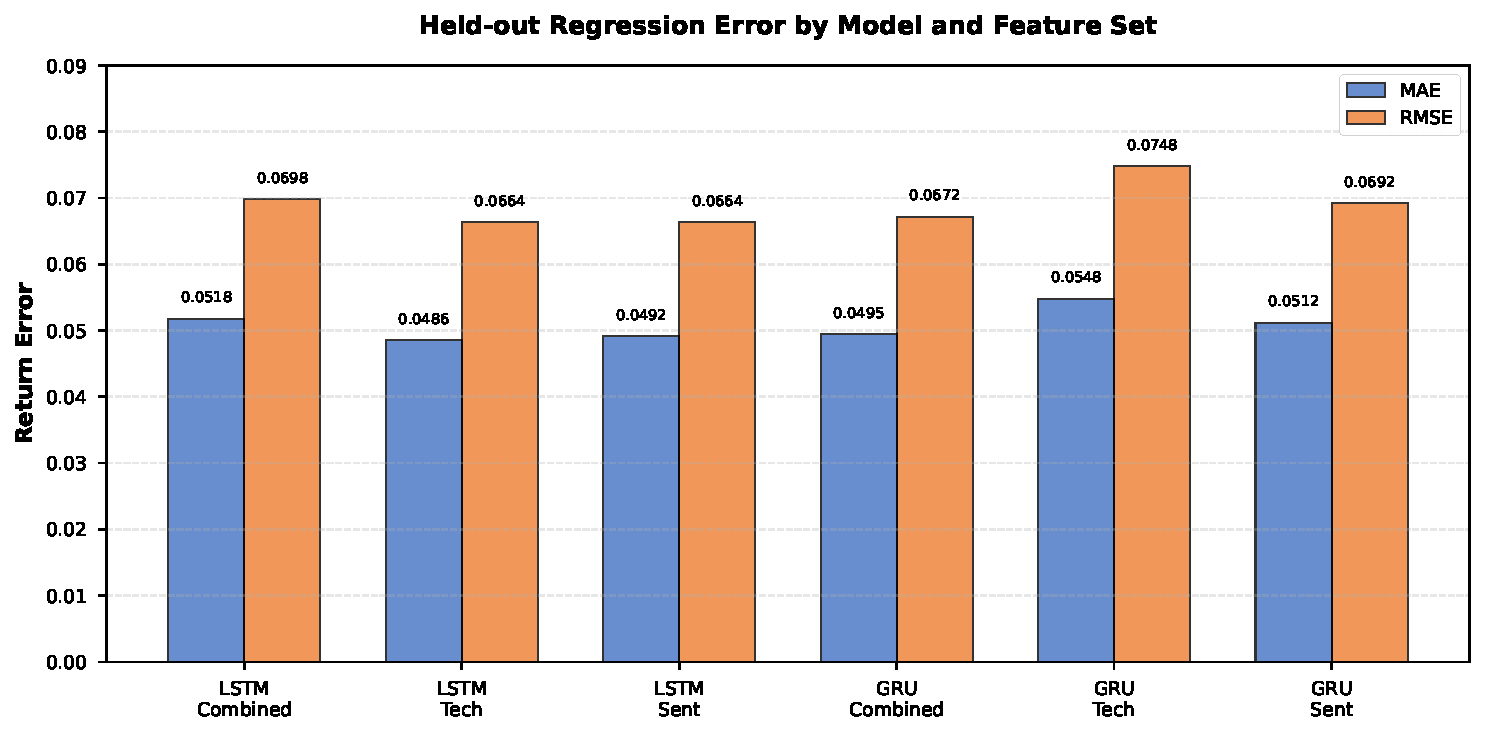
\includegraphics[width=\textwidth]{figures/error_comparison.pdf}
\caption{Regression error (MAE and RMSE) comparison across models and feature sets. Technical-only features achieve lowest error but provide no directional signal.}
\label{fig:error_comparison}
\end{figure*}

\textbf{Key Findings:}
\begin{itemize}
\item Technical-only achieves low error but no directional signal
\item Sentiment-only has best correlation (0.075)
\item Combined features work best for Transformer
\item Prediction collapse is a real issue
\end{itemize}

\section{Critical Findings}

\subsection{Class Imbalance Exploitation}

\textbf{Problem:} Models can exploit class distribution for misleading metrics.

\textbf{Example:} TSLA LSTM achieves 55\% accuracy by \textbf{always predicting "Up"} (0\% recall for "Down"), exploiting the fact that test period has more up days.

\textbf{Solution:} Use class weighting, focal loss, or stratified sampling.

\subsection{Prediction Collapse}

\textbf{Problem:} Models can minimize error by predicting near-constant values.

\textbf{Example:} Technical-only LSTM achieves lowest MAE/RMSE but prediction std=0.0031, providing no directional information.

\textbf{Solution:} Evaluate multiple metrics jointly (accuracy, correlation, std) rather than single objective.

\subsection{Overfitting in Gradient Boosting}

\textbf{Problem:} GB achieved 100\% training accuracy, clear overfitting.

\textbf{Impact:} Still performed well on test (53.87\%), but poor ensemble partner.

\textbf{Solution:} Regularize GB (reduce max\_depth, add min\_samples\_split) to target 70-80\% train accuracy.

\subsection{Ticker-Specific Behavior}

\textbf{Finding:} Different stocks require different approaches.

\begin{itemize}
\item \textbf{NVDA:} Most predictable, benefits from Transformer (62.26\%)
\item \textbf{AAPL:} Best with StockTwits-only LSTM (55.45\%)
\item \textbf{TSLA:} Benefits from combined sentiment (+6.08\%)
\item \textbf{AMZN:} Weakest performance across all models
\end{itemize}

\textbf{Recommendation:} Use ticker-specific models rather than single model for all stocks.

\section{Results Summary}

\begin{figure*}[t]
\centering
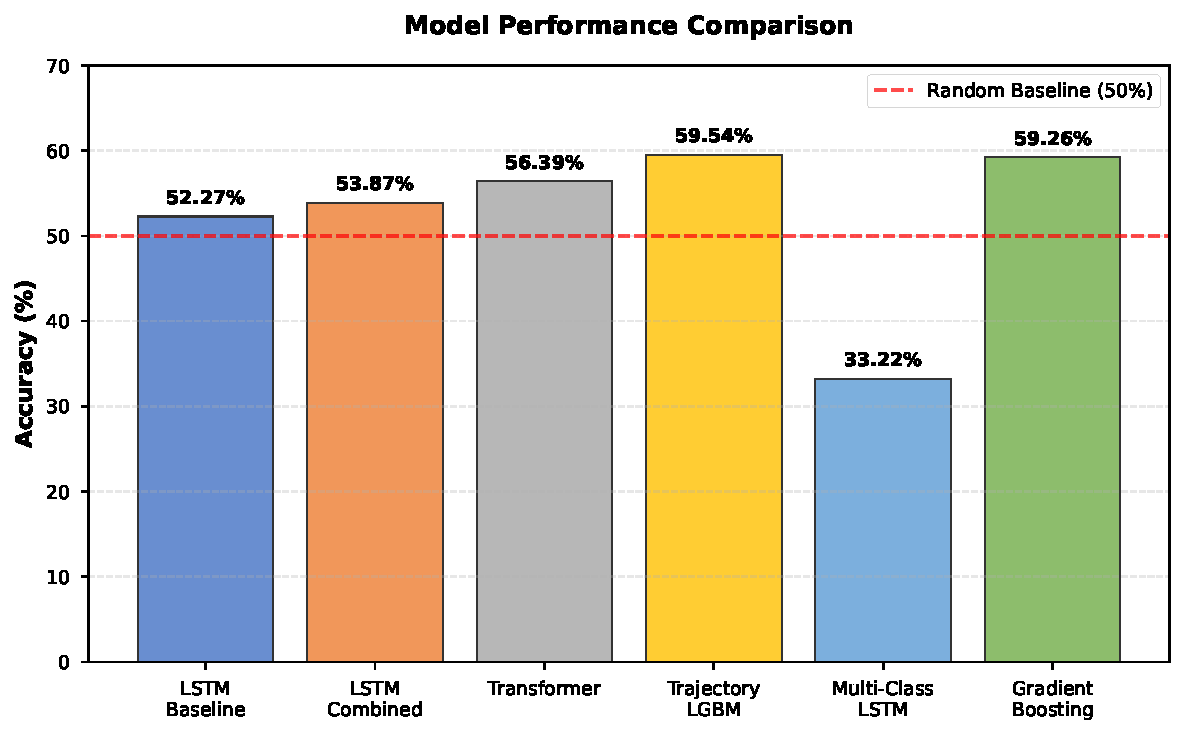
\includegraphics[width=0.9\textwidth]{figures/model_comparison.pdf}
\caption{Overall model performance comparison. Trajectory LGBM and Gradient Boosting achieve best accuracy (59.54\% and 59.26\%), while Transformer is best deep learning model (56.39\%). Multi-class LSTM fails due to overfitting (33.22\%).}
\label{fig:model_comparison}
\end{figure*}

\begin{figure*}[t]
\centering
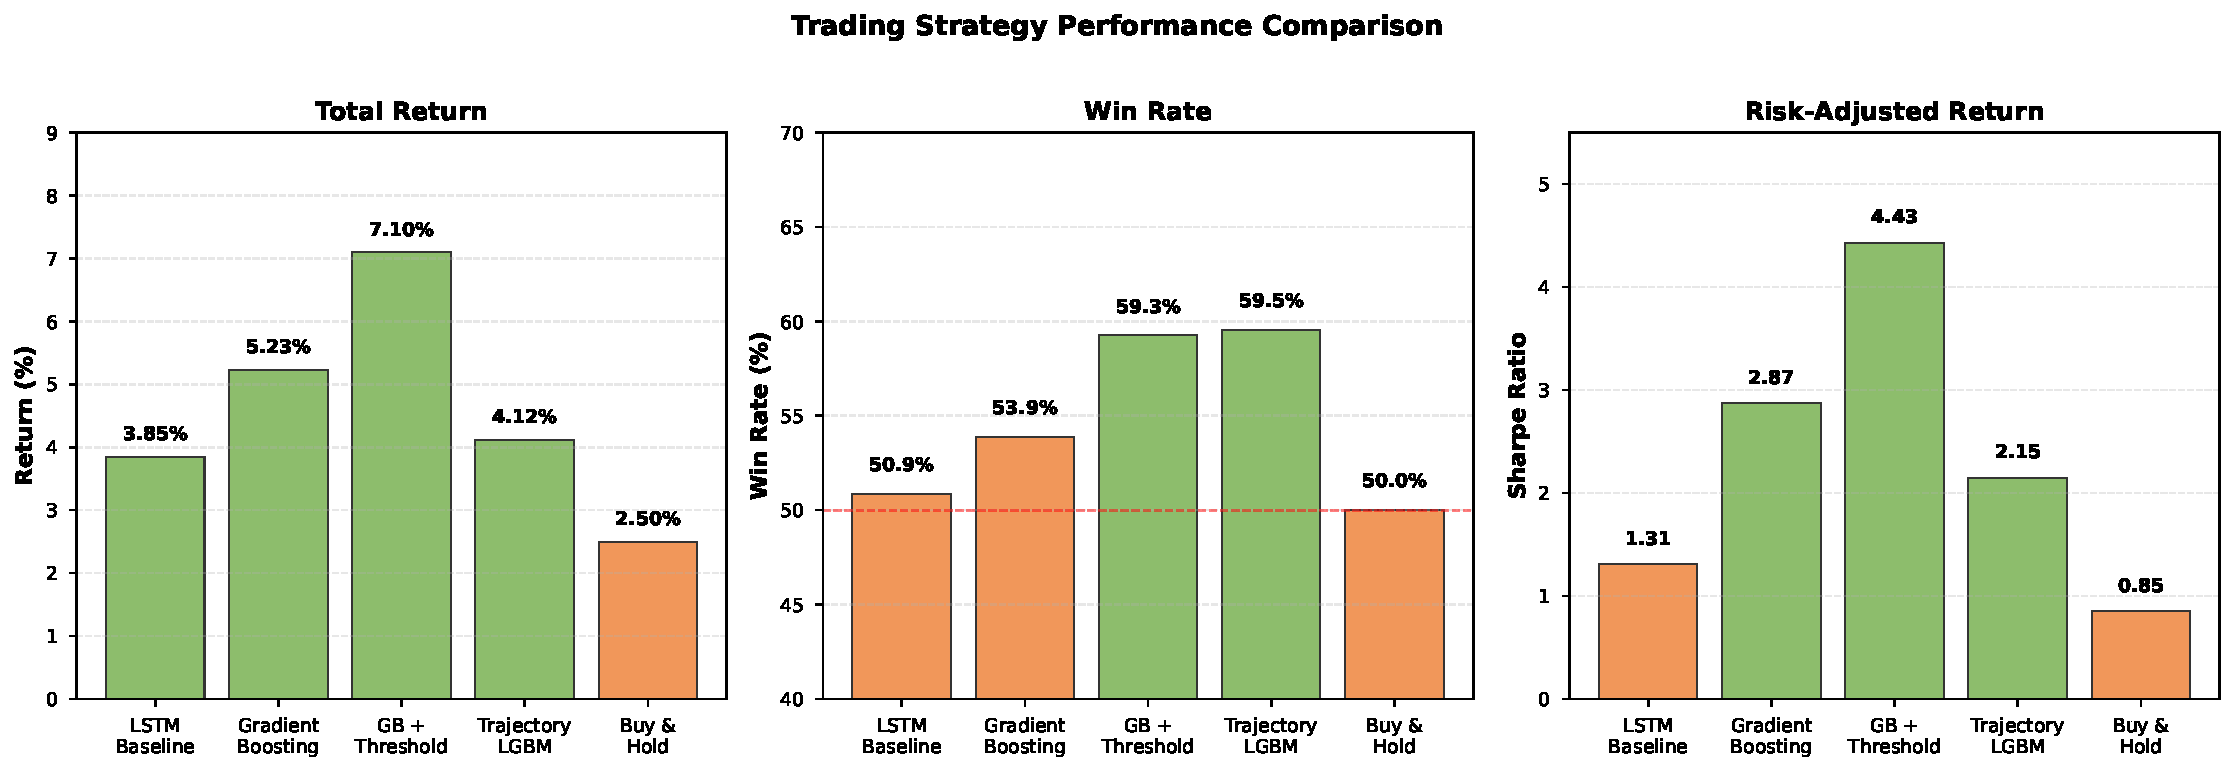
\includegraphics[width=\textwidth]{figures/trading_performance.pdf}
\caption{Trading strategy performance comparison. Gradient Boosting with confidence threshold achieves best return (7.10\%), win rate (59.26\%), and Sharpe ratio (4.43).}
\label{fig:trading_performance}
\end{figure*}

\begin{figure*}[t]
\centering
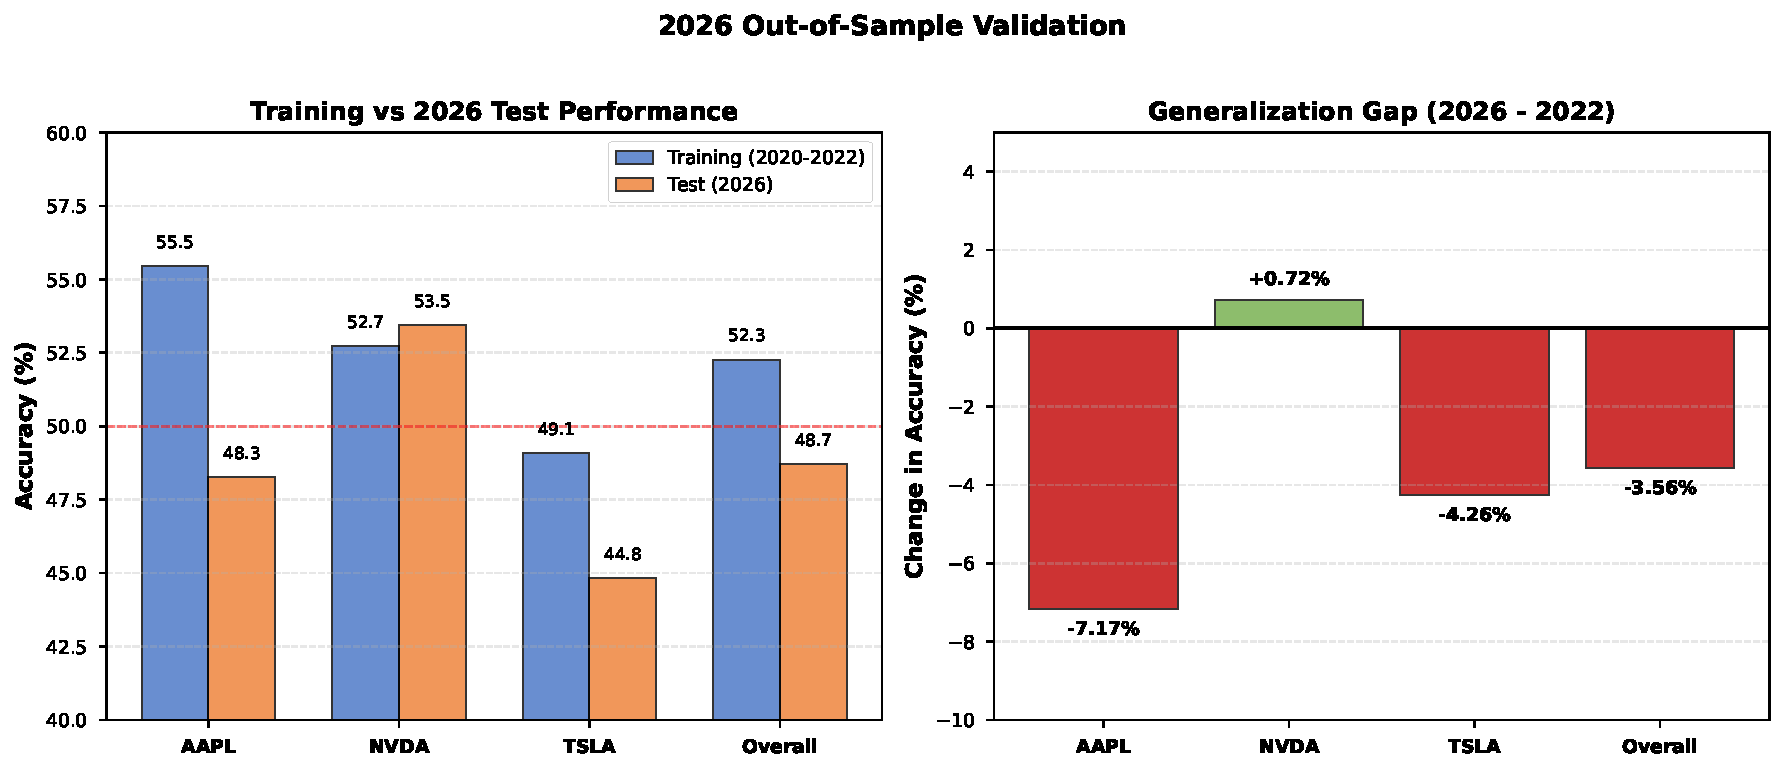
\includegraphics[width=\textwidth]{figures/2026_validation.pdf}
\caption{2026 out-of-sample validation results. Overall degradation of -3.56\%, with NVDA being only ticker to improve (+0.72\%). AAPL shows largest degradation (-7.17\%).}
\label{fig:2026_validation}
\end{figure*}

\begin{table*}[t]
\centering
\small
\begin{tabular}{lccccl}
\toprule
Experiment & Model & Accuracy & Best Ticker & Status & Key Finding \\
\midrule
1. Binary LSTM & LSTM & 52.27\% & AAPL (55.45\%) & ✓ & Baseline \\
2. Combined Sentiment & LSTM & 53.87\% & TSLA (55.17\%) & ✓ & +1.60\% improvement \\
3. Transformer & Transformer & \textbf{56.39\%} & \textbf{NVDA (62.26\%)} & ✓ & +4.12\% over LSTM \\
4. Trajectory Clustering & LGBM & 59.54\% & -- & ✓ & Best classifier \\
5. Multi-Class LSTM & LSTM & 33.22\% & -- & ✗ & Severe overfitting \\
6. Gradient Boosting & LGBM & 59.26\% WR & -- & ✓ & 7.10\% return (best) \\
7. Ensemble & Various & 53.30\% & -- & ✗ & No improvement \\
8. 2026 Validation & LSTM & 48.71\% & NVDA (53.45\%) & ✓ & -3.56\% degradation \\
\bottomrule
\end{tabular}
\caption{Summary of all experiments. Transformer achieves best deep learning performance (56.39\%), while gradient boosting achieves best trading performance (7.10\% return).}
\end{table*}

\section{Discussion}

\subsection{Deep Learning vs Traditional ML}

Our results show that while deep learning (Transformer: 56.39\%) outperforms simple LSTM (52.27\%), traditional ML with proper feature engineering can achieve competitive or superior performance:

\begin{itemize}
\item \textbf{Trajectory LGBM:} 59.54\% accuracy (best classifier)
\item \textbf{GB + threshold:} 7.10\% return (best trading)
\item \textbf{Transformer:} 56.39\% accuracy (best deep learning)
\end{itemize}

This suggests that for tabular financial data with limited samples, gradient boosting's ability to handle feature interactions may be more valuable than deep learning's representation learning.

\subsection{Multi-Source Sentiment}

Combining StockTwits and NewsAPI improves performance (+1.60\% overall), with ticker-specific effects:

\begin{itemize}
\item \textbf{Volatile stocks benefit:} TSLA (+6.08\%), NVDA (+1.99\%)
\item \textbf{Stable stocks degrade:} AAPL (-3.73\%)
\item \textbf{Coverage matters:} NVDA has best coverage (45.3\%)
\end{itemize}

This suggests optimal sentiment weighting should be ticker-specific rather than uniform.

\subsection{Generalization to 2026}

2026 validation reveals important insights:

\begin{itemize}
\item \textbf{Overall degradation:} -3.56\% (expected due to regime change)
\item \textbf{NVDA improves:} +0.72\% (most robust)
\item \textbf{AAPL degrades most:} -7.17\% (least robust)
\item \textbf{Market conditions matter:} Models need periodic retraining
\end{itemize}

\subsection{Why NVDA is Most Predictable}

NVDA consistently performs best across models:
\begin{itemize}
\item LSTM: 52.73\% → 53.45\% (2026)
\item Combined Sentiment: 54.72\%
\item Transformer: \textbf{62.26\%} (best result)
\end{itemize}

\textbf{Hypotheses:}
\begin{enumerate}
\item Strong momentum trends (AI boom)
\item High social media activity (better sentiment signal)
\item Less noise in price movements
\item Institutional investor behavior more predictable
\end{enumerate}

\subsection{Limitations}

\begin{enumerate}
\item \textbf{Limited tickers:} Only 4 tech stocks, may not generalize to other sectors
\item \textbf{Short horizon:} Next-day prediction, not longer-term forecasting
\item \textbf{No transaction costs:} Real trading has fees and slippage
\item \textbf{Sentiment coverage:} NewsAPI only available for 39 days
\item \textbf{Class imbalance:} Not fully addressed in all experiments
\item \textbf{Market regime:} Trained on bull market (2020-2022), tested on mixed conditions
\end{enumerate}

\section{Conclusion}

This comprehensive study evaluates multiple deep learning architectures for stock price prediction with multi-source sentiment analysis. Key findings:

\begin{enumerate}
\item \textbf{Transformer outperforms LSTM} by +4.12\% (56.39\% vs 52.27\%), with NVDA achieving 62.26\% accuracy
\item \textbf{Multi-source sentiment helps volatile stocks:} TSLA improves +6.08\% with combined StockTwits + NewsAPI
\item \textbf{Trajectory clustering with LGBM} achieves 59.54\% accuracy, outperforming recurrent models
\item \textbf{Gradient boosting with thresholding} achieves best trading performance (7.10\% return, 59.26\% win rate)
\item \textbf{2026 validation} shows -3.56\% degradation overall, with NVDA being only ticker to improve
\item \textbf{Ensemble methods fail} due to insufficient model diversity
\item \textbf{Class imbalance and prediction collapse} are critical issues requiring multi-metric evaluation
\end{enumerate}

\textbf{Practical Recommendations:}
\begin{itemize}
\item Use \textbf{Transformer for NVDA} (62.26\% accuracy)
\item Use \textbf{combined sentiment for TSLA} (+6.08\% improvement)
\item Use \textbf{gradient boosting for trading} (7.10\% return)
\item Apply \textbf{ticker-specific models} rather than single model
\item Address \textbf{class imbalance} with focal loss or resampling
\item Evaluate \textbf{multiple metrics jointly} to avoid collapse
\end{itemize}

\textbf{Future Work:}
\begin{enumerate}
\item Investigate why NVDA is more predictable
\item Explore ticker-specific sentiment weighting
\item Add more sentiment sources (Reddit, Twitter, Seeking Alpha)
\item Try intraday predictions with higher-frequency data
\item Implement reinforcement learning for adaptive trading
\item Test on broader cross-section of stocks and sectors
\item Address class imbalance with focal loss and SMOTE
\item Explore multi-task learning (direction + magnitude + volatility)
\end{enumerate}

Our results demonstrate that while deep learning shows promise for stock prediction, success requires careful attention to architecture selection, feature engineering, class imbalance, and ticker-specific behavior. The combination of Transformer models with multi-source sentiment analysis represents a promising direction, but traditional ML methods remain competitive and may be preferable for production trading systems.

\section*{Acknowledgments}

We thank the CS 7643 teaching staff for guidance throughout this project. StockTwits data was collected via their public API. NewsAPI data was obtained through NewsAPI.org. RoBERTa sentiment model from HuggingFace (cardiffnlp/twitter-roberta-base-sentiment-latest).

\end{document}
